\documentclass{article}

% Packages
\usepackage[english]{babel}
\usepackage[letterpaper,top=2cm,bottom=2cm,left=3cm,right=3cm,marginparwidth=1.75cm]{geometry}
\usepackage{amsmath}
\usepackage{graphicx}
\usepackage{float}
\usepackage[colorlinks=true, allcolors=blue]{hyperref}
\usepackage[parfill]{parskip}

\newcommand{\subsubsubsection}[1]{\paragraph{#1}\mbox{}\\}
\setcounter{secnumdepth}{4}
\setcounter{tocdepth}{4}

\title{AI References and Reading List}
\author{Michael Hollins}

\begin{document}
\maketitle

\section{Introduction}

An \href{http://varianceexplained.org/r/ds-ml-ai/}{oversimplified definition} of the differences between data science (DS), machine learning (ML) and artificial intelligence (AI) is that DS produces \textbf{insights}, ML produces \textbf{predictions}, and AI produces \textbf{actions}. There is no universally accepted definition of any of these terms, so choose whatever helps you conceptually and doesn't mislead others. For a slightly more detailed introduction into the landscape of AI and ML, see this \href{https://www.ml4devs.com/articles/machine-learning-intro-for-developers/}{blog}. In particular, this diagram explaining the difference between traditional programming and ML is helpful:

\begin{figure}[H]
    \centering
    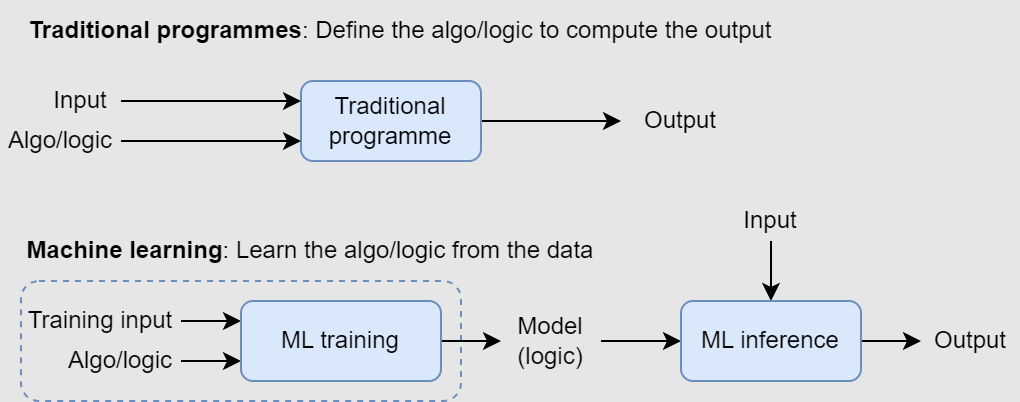
\includegraphics[width=\textwidth]{MLExplainer.png}
    \caption{Traditional programmes vs ML algorithms, source: \href{https://www.ml4devs.com/articles/machine-learning-intro-for-developers/}{Satish Chandra Gupta}}
    \label{fig:MLExplainer}
\end{figure}

\section{Machine Learning Books}

\begin{itemize}
    \item \href{https://link.springer.com/book/10.1007/978-0-387-84858-7}{The Elements of Statistical Learning}, by Hastie, Tibshirani, Friedman
    \item \href{https://www.statlearning.com/}{An Introduction to Statistical Learning}, by James, Witten, Hastie, Tibshirani
    \item \href{https://www.deeplearningbook.org/}{Deep Learning}, by Goodfellow, Bengio, Courville, Bach
    \item \href{https://www.microsoft.com/en-us/research/people/cmbishop/prml-book/}{Pattern Recognition and Machine Learning}, by Bishop
    \item \href{https://web.stanford.edu/~jurafsky/slp3/}{Speech and Language Processing}, by Jurafsky, Martin
\end{itemize}

\section{Video Lectures}

\textbf{Deep Learning: }\href{http://introtodeeplearning.com/}{MIT 6.2191} is a series of free lectures which provide a helpful introduction to deep learning from the MIT. The full series of lectures can be found \href{https://www.youtube.com/playlist?list=PLtBw6njQRU-rwp5__7C0oIVt26ZgjG9NI}{here}. The topics covered include neural networks, sequential modelling (including transformers), convolution neural networks, generative modelling, reinforcement learning, and language models. 

\section{Lecture Notes}
\begin{itemize}
    \item Machine Learning: \href{https://princeton-introml.github.io/files/COS324_Course_Notes.pdf}{Princeton}.
    \item Vector Calculus: \href{https://www.damtp.cam.ac.uk/user/tong/vc/vc.pdf}{Cambridge}, and \href{https://www.damtp.cam.ac.uk/user/tong/vc.html}{work sheets.}
    \item Machine Learning (actual lecture notes!): \href{https://people.eecs.berkeley.edu/~jrs/papers/machlearn.pdf}{UC Berkley}
\end{itemize}

\section{Core References}

This section introduces some of the most important papers in AI and ML.\footnote{Compiled using \href{https://www.perplexity.ai/search/i-want-a-list-of-the-most-impo-XR\_jbWnpQtqxWLKwizn6uQ\#0}{Perplexity}}

\subsection{Foundational Papers}

\subsubsection*{Computing Machinery and Intelligence}

``Computing Machinery and Intelligence'' by Alan Turing (1950) is a seminal \href{https://www.cs.ox.ac.uk/activities/ieg/e-library/sources/t_article.pdf}{paper} that laid the groundwork for artificial intelligence research.\cite{Turing1950} In this influential work, Turing proposes the famous Turing Test as a method to determine if a machine can exhibit intelligent behavior indistinguishable from a human. He introduces the concept of the "imitation game," where an interrogator attempts to distinguish between a human and a machine through a series of questions. Turing argues that if a machine can successfully fool the interrogator, it can be considered to be "thinking"[1]. The paper also addresses several objections to the idea of machine intelligence, including the "Lady Lovelace's Objection" regarding machine creativity. By reframing the question "Can machines think?" into a more concrete and testable format, Turing provided a foundation for future AI research and development.

\subsubsection*{A Logical Calculus of the Ideas Immanent in Nervous Activity}

``A Logical Calculus of the Ideas Immanent in Nervous Activity'' by Warren McCulloch and Walter Pitts (1943) is a groundbreaking \href{https://link.springer.com/article/10.1007/BF02478259}{paper} that laid the foundation for artificial neural networks and computational neuroscience.\cite{Mcculloch1943} The authors proposed a mathematical model of neural networks based on propositional logic, demonstrating that the "all-or-none" nature of neuronal firing could be represented using Boolean algebra. They showed that any logical expression could be implemented by a network of idealized neurons, and that such networks could perform complex computations. The paper introduced key concepts like threshold logic, temporal summation, and inhibition, which are still fundamental to our understanding of both biological and artificial neural networks. By bridging neurobiology and mathematical logic, McCulloch and Pitts provided a theoretical framework for understanding how the brain processes information and laid the groundwork for future developments in artificial intelligence and cognitive science.

\subsection{Machine Learning Algorithms}

\subsubsection*{A Decision-Theoretic Generalization of On-Line Learning and an Application to Boosting}

``A Decision-Theoretic Generalization of On-Line Learning and an Application to Boosting'' by Yoav Freund and Robert E. Schapire (1997) \href{https://www.face-rec.org/algorithms/Boosting-Ensemble/decision-theoretic_generalization.pdf}{introduced} the AdaBoost (Adaptive Boosting) algorithm.\cite{Freund1997} This is a powerful machine learning algorithm that combines multiple "weak" classifiers to create a strong classifier. The authors introduce a novel approach to boosting that adapts to the accuracies of the weak learners without requiring prior knowledge of their performance. AdaBoost works by iteratively reweighting the training data, focusing more on misclassified examples in each round. The algorithm then combines the weak classifiers into a final strong classifier using a weighted majority vote. The paper proves that AdaBoost can efficiently convert weak learning algorithms into strong ones, with the training error decreasing exponentially fast if each weak hypothesis is slightly better than random guessing. This work has had a profound impact on machine learning, leading to numerous applications and extensions in various fields.

\subsubsection*{Random Forests}

The paper ``Random Forests'' by Leo Breiman (2001) \href{https://link.springer.com/article/10.1023/A:1010933404324}{introduces} a novel ensemble learning method that combines multiple decision trees to create a robust and accurate classifier.\cite{Breiman2001} Key aspects of the algorithm include: Each tree is grown using a bootstrap sample of the training data; At each node, a random subset of features is selected for splitting; Trees are grown to maximum depth without pruning; Predictions are made by aggregating votes from all trees.

Breiman shows that the performance of Random Forests depends on two main factors: the strength of individual trees and the correlation between them. The paper provides theoretical analysis and empirical results demonstrating that Random Forests compare favorably to other ensemble methods like AdaBoost, especially in the presence of noise.

\subsubsection*{XGBoost: A Scalable Tree Boosting System}

The paper ``XGBoost: A Scalable Tree Boosting System'' by Tianqi Chen and Carlos Guestrin (2016) \href{https://arxiv.org/abs/1603.02754}{introduces} XGBoost, a highly efficient and flexible implementation of gradient boosting.\cite{Chen2016} Key aspects of the algorithm include:
\begin{itemize}
    \item A novel sparsity-aware algorithm for handling sparse data.
    \item A weighted quantile sketch for approximate tree learning.
    \item Cache-aware access patterns for out-of-core tree learning.
    \item Distributed computing for large-scale tree boosting.
\end{itemize}

The authors provide theoretical justification for the system's performance and present detailed benchmarks. They also highlight XGBoost's impact on machine learning competitions, where it has been widely used in winning solutions across various domains.

\subsubsection*{Support Vector Networks}

``Support Vector Networks'' by Corinna Cortes and Vladimir Vapnik (1995) is a seminal \href{https://link.springer.com/article/10.1007/BF00994018}{paper} that introduced Support Vector Machines (SVMs), a powerful machine learning algorithm for classification problems.\cite{Cortes1995} The authors present a novel approach to creating a decision boundary in a high-dimensional feature space, where input vectors are non-linearly mapped. The key innovation is the concept of support vectors - the subset of training points that lie closest to the decision surface. These support vectors are used to construct an optimal hyperplane that maximizes the margin between different classes. The paper extends the idea to handle non-separable training data by introducing soft margins, allowing for some misclassifications while still maximizing the margin. This approach significantly improved the generalization ability of the classifier, making SVMs highly effective for various real-world applications. The authors demonstrate the algorithm's performance on optical character recognition tasks, showcasing its superiority over classical learning algorithms of the time.

\subsection{Neural Networks and Deep Learning}

\subsubsection*{Gradient-Based Learning Applied to Document Recognition}

The paper ``Gradient-Based Learning Applied to Document Recognition'' by Yann LeCun, Léon Bottou, Yoshua Bengio, and Patrick Haffner (1998) is a landmark \href{https://ieeexplore.ieee.org/document/726791}{publication} in the field of neural networks and deep learning, particularly for introducing Convolutional Neural Networks (CNNs).\cite{Lecun1998} This comprehensive work presents a novel architecture specifically designed for processing 2D shapes with high variability, such as handwritten characters. The authors demonstrate the power of gradient-based learning techniques, particularly backpropagation, in training multilayer neural networks to classify high-dimensional patterns with minimal preprocessing. The paper introduces key concepts like local receptive fields, shared weights, and spatial subsampling, which are fundamental to CNNs. It also compares various methods for handwritten character recognition, showing that CNNs outperform other techniques of the time. Additionally, the authors present the Graph Transformer Network (GTN) paradigm, allowing for global training of multi-module systems using gradient-based methods. The work's impact is evident in its applications to real-world document recognition systems, including a commercially deployed check-reading system.

\subsubsection*{ImageNet Classification with Deep Convolutional Neural Networks}

``ImageNet Classification with Deep Convolutional Neural Networks'' by Alex Krizhevsky, Ilya Sutskever, and Geoffrey E. Hinton (2012) \href{https://papers.nips.cc/paper/2012/file/c399862d3b9d6b76c8436e924a68c45b-Paper.pdf}{introduced} AlexNet, a deep convolutional neural network that achieved remarkable performance on the ImageNet Large Scale Visual Recognition Challenge (ILSVRC) in 2012.\cite{Krizhevsky2012} The authors demonstrated the power of deep learning for large-scale image classification, significantly outperforming previous state-of-the-art methods. Key innovations in this paper include:
\begin{enumerate}
    \item The use of ReLU (Rectified Linear Unit) activation functions, which allowed for faster training of deep networks.
    \item Implementation of data augmentation techniques to reduce overfitting.
    \item Dropout regularization to further combat overfitting in large networks.
    \item Local response normalization to aid generalization.
    \item Overlapping pooling to reduce the size of the network.
\end{enumerate}

The success of AlexNet on the ImageNet dataset, which contained over a million images in 1000 categories, marked a turning point in computer vision and deep learning. It demonstrated that deep convolutional neural networks could effectively learn hierarchical features from large-scale datasets, leading to significant improvements in image classification accuracy. This paper sparked renewed interest in deep learning and paved the way for numerous advancements in the field.

\subsubsection*{Long Short-Term Memory}

The paper "Long Short-Term Memory" by Sepp Hochreiter and Jürgen Schmidhuber (1997) \href{https://www.researchgate.net/publication/13853244_Long_Short-term_Memory}{introduced} the Long Short-Term Memory (LSTM) architecture, a significant advancement in recurrent neural networks (RNNs).\cite{Hochreiter1997} LSTMs were designed to address the vanishing gradient problem that plagued traditional RNNs, allowing them to learn long-term dependencies in sequential data. The key innovation of LSTMs is the introduction of a memory cell with gating mechanisms:
\begin{enumerate}
    \item The input gate controls what new information is added to the cell state.
    \item The forget gate determines what information should be discarded from the cell state.
    \item The output gate decides what information from the cell state should be output.
\end{enumerate}

These gates allow LSTMs to selectively remember or forget information over long sequences, making them particularly effective for tasks involving time series data, natural language processing, and speech recognition. The paper demonstrated the LSTM's ability to solve complex, artificial long-time-lag tasks that traditional RNNs could not handle. This architecture has since become a cornerstone in many sequence modeling tasks and has inspired numerous variants and improvements in the field of deep learning.

\subsection{Natural Language Processing}

\subsubsection*{Attention Is All You Need}

The paper ``Attention Is All You Need'' by Vaswani et al. (2017) \href{https://arxiv.org/pdf/1706.03762}{introduced} the Transformer architecture, a groundbreaking approach to sequence transduction that relies entirely on attention mechanisms.\cite{Vaswani2017} This model dispensed with recurrence and convolutions, which were previously considered essential for state-of-the-art performance in tasks like machine translation. The key innovations of the Transformer include:
\begin{enumerate}
    \item Multi-head self-attention: Allowing the model to jointly attend to information from different representation subspaces at different positions.
    \item Positional encoding: Injecting information about the relative or absolute position of tokens in the sequence.
    \item Scaled dot-product attention: An efficient attention mechanism that computes the attention weights using queries, keys, and values.
    \item Layer normalization and residual connections: Techniques to stabilize the training of deep networks.
\end{enumerate}

The Transformer architecture demonstrated superior performance on machine translation tasks while being more parallelisable and requiring significantly less training time compared to recurrent or convolutional models. This paper has had a profound impact on the field of natural language processing, serving as the foundation for many subsequent models like BERT, GPT, and T5, which have achieved state-of-the-art results across a wide range of NLP tasks.

\subsubsection*{BERT: Pre-training of Deep Bidirectional Transformers for Language Understanding}

The paper ``BERT: Pre-training of Deep Bidirectional Transformers for Language Understanding'' by Jacob Devlin, Ming-Wei Chang, Kenton Lee, and Kristina Toutanova (2019) \href{https://aclanthology.org/N19-1423/}{introduced} BERT (Bidirectional Encoder Representations from Transformers), a groundbreaking language representation model.\cite{Devlin2019} BERT's key innovation is its ability to pre-train deep bidirectional representations from unlabeled text by jointly conditioning on both left and right context in all layers. This approach differs from previous models that were either unidirectional or shallowly bidirectional.
Key aspects of BERT include:
\begin{enumerate}
    \item Masked Language Model (MLM) pre-training: Randomly masking some tokens in the input and predicting them based on context.
    \item Next Sentence Prediction (NSP): Pre-training text-pair representations to understand relationships between sentences.
    \item Fine-tuning: The pre-trained BERT model can be fine-tuned with just one additional output layer for various NLP tasks.
    \item Transformer architecture: Utilizing the powerful Transformer encoder for processing input text.
\end{enumerate}

BERT achieved state-of-the-art results on eleven NLP tasks, including significant improvements on the GLUE benchmark, MultiNLI, and SQuAD. Its success demonstrated the power of unsupervised pre-training and transfer learning in NLP, paving the way for a new paradigm in language understanding models.

\subsubsection*{Understanding LLMs: A Comprehensive Overview from Training to Inference}

The paper ``Understanding LLMs: A Comprehensive Overview from Training to Inference'' by Yiheng Liu et al. (2024) \href{https://arxiv.org/abs/2401.02038}{provides} a comprehensive review of Large Language Models (LLMs), focusing on cost-efficient training and deployment techniques. The authors present an overview of the evolution of LLM training and inference deployment technologies, addressing the increasing demand for more efficient approaches in the wake of ChatGPT's popularity. Key aspects covered in the paper include training techniques, inference deployment, and future trends.

This work serves as a valuable resource for researchers and practitioners in the field of natural language processing, offering a holistic view of the current state and future directions of LLM technology, with a particular emphasis on efficiency and scalability.

\subsection{Reinforcement Learning}

\subsubsection*{Playing Atari with Deep Reinforcement Learning}

The paper ``Playing Atari with Deep Reinforcement Learning'' by Volodymyr Mnih et al. (2013) \href{https://arxiv.org/abs/1312.5602}{introduced} the first deep learning model to successfully learn control policies directly from high-dimensional sensory input using reinforcement learning.\cite{Mnih2013} This groundbreaking work applied deep reinforcement learning to Atari 2600 games, demonstrating that a single architecture could learn to play multiple games without game-specific adjustments.
Key innovations and features of this paper include:
\begin{enumerate}
    \item Use of a convolutional neural network (CNN) to process raw pixel input from Atari games.
    \item Application of Q-learning with experience replay to train the network.
    \item End-to-end learning of game strategies without hand-crafted features or game-specific information.
    \item Consistent architecture and hyperparameters across multiple games.
    \item Introduction of the Deep Q-Network (DQN) algorithm.
    \item Outperforming previous approaches on six out of seven Atari games tested.
    \item Surpassing human expert performance on three games.
\end{enumerate}

This work laid the foundation for deep reinforcement learning in complex environments and sparked a new wave of research in applying deep learning to reinforcement learning problems. It demonstrated the potential of neural networks to learn effective policies directly from high-dimensional sensory inputs, paving the way for advancements in areas such as robotics, autonomous systems, and game AI.

\subsubsection*{Human-level Control through Deep Reinforcement Learning}

The paper ``Human-level control through deep reinforcement learning'' by Volodymyr Mnih et al. (2015) \href{https://www.semanticscholar.org/paper/Human-level-control-through-deep-reinforcement-Mnih-Kavukcuoglu/340f48901f72278f6bf78a04ee5b01df208cc508}{represents} a significant advancement in deep reinforcement learning, building upon their previous work on playing Atari games.\cite{Mnih2015} This study introduced the Deep Q-Network (DQN) agent, which achieved human-level performance across a wide range of Atari 2600 games.
Key innovations and findings of this paper include:
\begin{enumerate}
    \item Stable learning of action-value functions using a deep neural network as a function approximator.
    \item Introduction of experience replay, which randomizes over data to remove correlations in the observation sequence and smooths over changes in the data distribution.
    \item Use of a target network to reduce correlations with the target, further stabilizing learning.
    \item Application of the same network architecture and hyperparameters across 49 different Atari games.
    \item Demonstration of human-level or superhuman performance on 29 of the 49 games tested.
    \item Ability to learn directly from high-dimensional sensory inputs (raw pixels) without manual feature engineering.
    \item Analysis of the learned representations, showing that the model learns human-interpretable features of the game states.
\end{enumerate}

This work significantly advanced the field of deep reinforcement learning by showing that a single architecture could learn to excel at a diverse array of challenging tasks, bridging the gap between high-dimensional sensory inputs and actions.

\subsection{Generative Models}

\subsubsection*{Generative Adversarial Networks}

The paper ``Generative Adversarial Nets'' by Ian Goodfellow et al. (2014) \href{https://arxiv.org/abs/1406.2661}{introduced} the concept of Generative Adversarial Networks (GANs), a revolutionary framework for training generative models.\cite{Goodfellow2014} This seminal work proposed a novel approach to estimating generative models via an adversarial process, where two models are simultaneously trained.

Key innovations and features of this paper include:
\begin{enumerate}
    \item Introduction of the GAN framework: A generative model G that captures the data distribution, and a discriminative model D that estimates the probability that a sample came from the training data rather than G.
    \item Adversarial training process: G is trained to maximize the probability of D making a mistake, while D is trained to accurately distinguish between real and generated samples.
    \item Formulation as a minimax two-player game: This game-theoretic approach ensures continuous improvement of both networks.
    \item Theoretical analysis: Proving the existence of a unique solution where G recovers the training data distribution and D equals 1/2 everywhere.
    \item Implementation using multilayer perceptrons: Demonstrating that the entire system can be trained with backpropagation.
    \item No need for Markov chains or unrolled approximate inference networks: Simplifying the training and generation process.
    \item Qualitative and quantitative evaluation: Demonstrating the potential of GANs through experiments on various datasets.
\end{enumerate}

This work has had a profound impact on the field of machine learning, particularly in image generation, and has sparked numerous extensions and applications across various domains.

\subsubsection*{Auto-Encoding Variational Bayes}

The paper ``Auto-Encoding Variational Bayes'' by Diederik P. Kingma and Max Welling \href{https://arxiv.org/abs/1312.6114}{introduces} a novel approach to perform efficient inference and learning in directed probabilistic models with continuous latent variables and intractable posterior distributions.\cite{Kingma2013} The authors present two main contributions:
\begin{enumerate}
    \item A reparameterization of the variational lower bound that yields a lower bound estimator which can be optimized using standard stochastic gradient methods.
    \item An efficient method for posterior inference in i.i.d. datasets with continuous latent variables per datapoint, by fitting an approximate inference model (recognition model) to the intractable posterior using the proposed lower bound estimator.
\end{enumerate}

The paper introduces the Auto-Encoding Variational Bayes (AEVB) algorithm, which makes inference and learning particularly efficient by using the Stochastic Gradient Variational Bayes (SGVB) estimator. This approach allows for very efficient approximate posterior inference using simple ancestral sampling, enabling efficient learning of model parameters without the need for expensive iterative inference schemes per datapoint.

The authors demonstrate the theoretical advantages of their method and provide experimental results that reflect these advantages. This work has had a significant impact on the field of machine learning, particularly in the development of variational autoencoders (VAEs) and other generative models.

\section{Other Useful References}

Imperial's Python course by the venerable \href{https://python.pages.doc.ic.ac.uk/}{Josiah Wang}.

\clearpage
\bibliographystyle{alpha}
\bibliography{sample}

\end{document}